% Options for packages loaded elsewhere
\PassOptionsToPackage{unicode}{hyperref}
\PassOptionsToPackage{hyphens}{url}
\PassOptionsToPackage{dvipsnames,svgnames,x11names}{xcolor}
%
\documentclass[
  letterpaper,
  DIV=11,
  numbers=noendperiod]{scrartcl}

\usepackage{amsmath,amssymb}
\usepackage{lmodern}
\usepackage{iftex}
\ifPDFTeX
  \usepackage[T1]{fontenc}
  \usepackage[utf8]{inputenc}
  \usepackage{textcomp} % provide euro and other symbols
\else % if luatex or xetex
  \usepackage{unicode-math}
  \defaultfontfeatures{Scale=MatchLowercase}
  \defaultfontfeatures[\rmfamily]{Ligatures=TeX,Scale=1}
\fi
% Use upquote if available, for straight quotes in verbatim environments
\IfFileExists{upquote.sty}{\usepackage{upquote}}{}
\IfFileExists{microtype.sty}{% use microtype if available
  \usepackage[]{microtype}
  \UseMicrotypeSet[protrusion]{basicmath} % disable protrusion for tt fonts
}{}
\makeatletter
\@ifundefined{KOMAClassName}{% if non-KOMA class
  \IfFileExists{parskip.sty}{%
    \usepackage{parskip}
  }{% else
    \setlength{\parindent}{0pt}
    \setlength{\parskip}{6pt plus 2pt minus 1pt}}
}{% if KOMA class
  \KOMAoptions{parskip=half}}
\makeatother
\usepackage{xcolor}
\setlength{\emergencystretch}{3em} % prevent overfull lines
\setcounter{secnumdepth}{-\maxdimen} % remove section numbering
% Make \paragraph and \subparagraph free-standing
\ifx\paragraph\undefined\else
  \let\oldparagraph\paragraph
  \renewcommand{\paragraph}[1]{\oldparagraph{#1}\mbox{}}
\fi
\ifx\subparagraph\undefined\else
  \let\oldsubparagraph\subparagraph
  \renewcommand{\subparagraph}[1]{\oldsubparagraph{#1}\mbox{}}
\fi

\usepackage{color}
\usepackage{fancyvrb}
\newcommand{\VerbBar}{|}
\newcommand{\VERB}{\Verb[commandchars=\\\{\}]}
\DefineVerbatimEnvironment{Highlighting}{Verbatim}{commandchars=\\\{\}}
% Add ',fontsize=\small' for more characters per line
\usepackage{framed}
\definecolor{shadecolor}{RGB}{241,243,245}
\newenvironment{Shaded}{\begin{snugshade}}{\end{snugshade}}
\newcommand{\AlertTok}[1]{\textcolor[rgb]{0.68,0.00,0.00}{#1}}
\newcommand{\AnnotationTok}[1]{\textcolor[rgb]{0.37,0.37,0.37}{#1}}
\newcommand{\AttributeTok}[1]{\textcolor[rgb]{0.40,0.45,0.13}{#1}}
\newcommand{\BaseNTok}[1]{\textcolor[rgb]{0.68,0.00,0.00}{#1}}
\newcommand{\BuiltInTok}[1]{\textcolor[rgb]{0.00,0.23,0.31}{#1}}
\newcommand{\CharTok}[1]{\textcolor[rgb]{0.13,0.47,0.30}{#1}}
\newcommand{\CommentTok}[1]{\textcolor[rgb]{0.37,0.37,0.37}{#1}}
\newcommand{\CommentVarTok}[1]{\textcolor[rgb]{0.37,0.37,0.37}{\textit{#1}}}
\newcommand{\ConstantTok}[1]{\textcolor[rgb]{0.56,0.35,0.01}{#1}}
\newcommand{\ControlFlowTok}[1]{\textcolor[rgb]{0.00,0.23,0.31}{#1}}
\newcommand{\DataTypeTok}[1]{\textcolor[rgb]{0.68,0.00,0.00}{#1}}
\newcommand{\DecValTok}[1]{\textcolor[rgb]{0.68,0.00,0.00}{#1}}
\newcommand{\DocumentationTok}[1]{\textcolor[rgb]{0.37,0.37,0.37}{\textit{#1}}}
\newcommand{\ErrorTok}[1]{\textcolor[rgb]{0.68,0.00,0.00}{#1}}
\newcommand{\ExtensionTok}[1]{\textcolor[rgb]{0.00,0.23,0.31}{#1}}
\newcommand{\FloatTok}[1]{\textcolor[rgb]{0.68,0.00,0.00}{#1}}
\newcommand{\FunctionTok}[1]{\textcolor[rgb]{0.28,0.35,0.67}{#1}}
\newcommand{\ImportTok}[1]{\textcolor[rgb]{0.00,0.46,0.62}{#1}}
\newcommand{\InformationTok}[1]{\textcolor[rgb]{0.37,0.37,0.37}{#1}}
\newcommand{\KeywordTok}[1]{\textcolor[rgb]{0.00,0.23,0.31}{#1}}
\newcommand{\NormalTok}[1]{\textcolor[rgb]{0.00,0.23,0.31}{#1}}
\newcommand{\OperatorTok}[1]{\textcolor[rgb]{0.37,0.37,0.37}{#1}}
\newcommand{\OtherTok}[1]{\textcolor[rgb]{0.00,0.23,0.31}{#1}}
\newcommand{\PreprocessorTok}[1]{\textcolor[rgb]{0.68,0.00,0.00}{#1}}
\newcommand{\RegionMarkerTok}[1]{\textcolor[rgb]{0.00,0.23,0.31}{#1}}
\newcommand{\SpecialCharTok}[1]{\textcolor[rgb]{0.37,0.37,0.37}{#1}}
\newcommand{\SpecialStringTok}[1]{\textcolor[rgb]{0.13,0.47,0.30}{#1}}
\newcommand{\StringTok}[1]{\textcolor[rgb]{0.13,0.47,0.30}{#1}}
\newcommand{\VariableTok}[1]{\textcolor[rgb]{0.07,0.07,0.07}{#1}}
\newcommand{\VerbatimStringTok}[1]{\textcolor[rgb]{0.13,0.47,0.30}{#1}}
\newcommand{\WarningTok}[1]{\textcolor[rgb]{0.37,0.37,0.37}{\textit{#1}}}

\providecommand{\tightlist}{%
  \setlength{\itemsep}{0pt}\setlength{\parskip}{0pt}}\usepackage{longtable,booktabs,array}
\usepackage{calc} % for calculating minipage widths
% Correct order of tables after \paragraph or \subparagraph
\usepackage{etoolbox}
\makeatletter
\patchcmd\longtable{\par}{\if@noskipsec\mbox{}\fi\par}{}{}
\makeatother
% Allow footnotes in longtable head/foot
\IfFileExists{footnotehyper.sty}{\usepackage{footnotehyper}}{\usepackage{footnote}}
\makesavenoteenv{longtable}
\usepackage{graphicx}
\makeatletter
\def\maxwidth{\ifdim\Gin@nat@width>\linewidth\linewidth\else\Gin@nat@width\fi}
\def\maxheight{\ifdim\Gin@nat@height>\textheight\textheight\else\Gin@nat@height\fi}
\makeatother
% Scale images if necessary, so that they will not overflow the page
% margins by default, and it is still possible to overwrite the defaults
% using explicit options in \includegraphics[width, height, ...]{}
\setkeys{Gin}{width=\maxwidth,height=\maxheight,keepaspectratio}
% Set default figure placement to htbp
\makeatletter
\def\fps@figure{htbp}
\makeatother

\usepackage{booktabs}
\usepackage{siunitx}

  \newcolumntype{d}{S[
    input-open-uncertainty=,
    input-close-uncertainty=,
    parse-numbers = false,
    table-align-text-pre=false,
    table-align-text-post=false
  ]}
  
\usepackage{longtable}
\usepackage{array}
\usepackage{multirow}
\usepackage{wrapfig}
\usepackage{float}
\usepackage{colortbl}
\usepackage{pdflscape}
\usepackage{tabu}
\usepackage{threeparttable}
\usepackage{threeparttablex}
\usepackage[normalem]{ulem}
\usepackage{makecell}
\usepackage{xcolor}
\KOMAoption{captions}{tableheading}
\makeatletter
\makeatother
\makeatletter
\makeatother
\makeatletter
\@ifpackageloaded{caption}{}{\usepackage{caption}}
\AtBeginDocument{%
\ifdefined\contentsname
  \renewcommand*\contentsname{Table of contents}
\else
  \newcommand\contentsname{Table of contents}
\fi
\ifdefined\listfigurename
  \renewcommand*\listfigurename{List of Figures}
\else
  \newcommand\listfigurename{List of Figures}
\fi
\ifdefined\listtablename
  \renewcommand*\listtablename{List of Tables}
\else
  \newcommand\listtablename{List of Tables}
\fi
\ifdefined\figurename
  \renewcommand*\figurename{Figure}
\else
  \newcommand\figurename{Figure}
\fi
\ifdefined\tablename
  \renewcommand*\tablename{Table}
\else
  \newcommand\tablename{Table}
\fi
}
\@ifpackageloaded{float}{}{\usepackage{float}}
\floatstyle{ruled}
\@ifundefined{c@chapter}{\newfloat{codelisting}{h}{lop}}{\newfloat{codelisting}{h}{lop}[chapter]}
\floatname{codelisting}{Listing}
\newcommand*\listoflistings{\listof{codelisting}{List of Listings}}
\makeatother
\makeatletter
\@ifpackageloaded{caption}{}{\usepackage{caption}}
\@ifpackageloaded{subcaption}{}{\usepackage{subcaption}}
\makeatother
\makeatletter
\@ifpackageloaded{tcolorbox}{}{\usepackage[many]{tcolorbox}}
\makeatother
\makeatletter
\@ifundefined{shadecolor}{\definecolor{shadecolor}{rgb}{.97, .97, .97}}
\makeatother
\makeatletter
\makeatother
\ifLuaTeX
  \usepackage{selnolig}  % disable illegal ligatures
\fi
\IfFileExists{bookmark.sty}{\usepackage{bookmark}}{\usepackage{hyperref}}
\IfFileExists{xurl.sty}{\usepackage{xurl}}{} % add URL line breaks if available
\urlstyle{same} % disable monospaced font for URLs
\hypersetup{
  pdftitle={Exploratory analysis of the RAND Health Insurance Experiment (HIE) data},
  pdfauthor={EB},
  colorlinks=true,
  linkcolor={blue},
  filecolor={Maroon},
  citecolor={Blue},
  urlcolor={Blue},
  pdfcreator={LaTeX via pandoc}}

\title{Exploratory analysis of the RAND Health Insurance Experiment
(HIE) data}
\author{EB}
\date{2023-05-02}

\begin{document}
\maketitle
\ifdefined\Shaded\renewenvironment{Shaded}{\begin{tcolorbox}[breakable, sharp corners, frame hidden, enhanced, borderline west={3pt}{0pt}{shadecolor}, boxrule=0pt, interior hidden]}{\end{tcolorbox}}\fi

\hypertarget{introduction}{%
\subsection{Introduction}\label{introduction}}

The RAND Health Insurance Experiment (HIE), which ran from 1974 to 1982,
was one of the most influential social experiments in research history.
It's purpose was to evaluate the price elasticity of the health
insurance plans. The HIE enrolled 3,958 people aged 14 to 61 from six
areas of the USA. The results of this randomized experiment could be
used for evaluating the causal effect of the health insurance on peoples
health.

Data that we are using in greater details is described in the Chapter 1.
Randomized Trials in
\href{https://hds.hebis.de/ubgi/Record/HEB35797798X}{Angrist, J. D., \&
Pischke, J.-S. (2014). Mastering'metrics: The path from cause to effect.
Princeton University Press.}. For our exercise, we use a somehow
simplified data set with only two distinct insurance plans:

\begin{enumerate}
\def\labelenumi{\arabic{enumi}.}
\tightlist
\item
  Catastrophic - Analogy of having no insurance
\item
  Free - the most comprehensive insurance plan that allows practically
  any medical treatment for free.
\end{enumerate}

The question that we want to answer is about the causal effect of
insurance of enrolled people health.

\begin{quote}
Note. To better understand the context, read subsection ``Randomized
results'' of the Chapter 1 in Mastering'metrics.
\end{quote}

\hypertarget{excersise-takaways}{%
\subsubsection{Excersise takaways:}\label{excersise-takaways}}

These are the key R-related skills showcased in this exercise;

\begin{enumerate}
\def\labelenumi{\arabic{enumi}.}
\item
  Data wrangling with:

  \begin{itemize}
  \tightlist
  \item
    \texttt{dplyr::filter()};
  \item
    \texttt{dplyr::select()};
  \end{itemize}
\item
  Descriptive statistics:

  \begin{itemize}
  \tightlist
  \item
    \texttt{mean()}, \texttt{sd()};
  \item
    \texttt{modelsummary::datasummary\_skim()};
  \end{itemize}
\item
  Means comparison:

  \begin{itemize}
  \tightlist
  \item
    \texttt{t.test()};
  \item
    \texttt{modelsummary::datasummary\_balance()}
  \item
    \texttt{lm()} - regression methods
  \end{itemize}
\item
  Causal effects analysis:

  \begin{itemize}
  \tightlist
  \item
    \texttt{t.test()};
  \item
    \texttt{modelsummary::datasummary\_balance()}
  \item
    \texttt{lm()}
  \end{itemize}
\end{enumerate}

\hypertarget{loading-packages-and-the-data}{%
\subsection{Loading packages and the
data}\label{loading-packages-and-the-data}}

To start working in R, we need to load packages. Sometimes, when we have
a fresh new version of R, we need to install libraries before loading
them. To install package, one need to run:
\texttt{install.packages("name\_of\_the\_package")}.

\begin{Shaded}
\begin{Highlighting}[]
\CommentTok{\# install.packages("psych")   }
\FunctionTok{library}\NormalTok{(psych)}

\CommentTok{\# install.packages("tidyverse")}
\FunctionTok{library}\NormalTok{(tidyverse)  }
\end{Highlighting}
\end{Shaded}

\begin{verbatim}
-- Attaching packages --------------------------------------- tidyverse 1.3.2 --
v ggplot2 3.4.2      v purrr   1.0.1 
v tibble  3.1.8      v dplyr   1.0.10
v tidyr   1.3.0      v stringr 1.5.0 
v readr   2.1.3      v forcats 0.5.2 
\end{verbatim}

\begin{verbatim}
Warning: package 'ggplot2' was built under R version 4.2.3
\end{verbatim}

\begin{verbatim}
Warning: package 'tidyr' was built under R version 4.2.3
\end{verbatim}

\begin{verbatim}
Warning: package 'purrr' was built under R version 4.2.3
\end{verbatim}

\begin{verbatim}
-- Conflicts ------------------------------------------ tidyverse_conflicts() --
x ggplot2::%+%()   masks psych::%+%()
x ggplot2::alpha() masks psych::alpha()
x dplyr::filter()  masks stats::filter()
x dplyr::lag()     masks stats::lag()
\end{verbatim}

\begin{Shaded}
\begin{Highlighting}[]
\CommentTok{\# install.packages("modelsummary")}
\FunctionTok{library}\NormalTok{(modelsummary)  }
\end{Highlighting}
\end{Shaded}

\begin{verbatim}

Attaching package: 'modelsummary'

The following object is masked from 'package:psych':

    SD
\end{verbatim}

\begin{Shaded}
\begin{Highlighting}[]
\CommentTok{\# install.packages("GGally")}
\FunctionTok{library}\NormalTok{(GGally)  }
\end{Highlighting}
\end{Shaded}

\begin{verbatim}
Warning: package 'GGally' was built under R version 4.2.3
\end{verbatim}

\begin{verbatim}
Registered S3 method overwritten by 'GGally':
  method from   
  +.gg   ggplot2
\end{verbatim}

Loading data

\begin{Shaded}
\begin{Highlighting}[]
\NormalTok{pre\_dta }\OtherTok{\textless{}{-}} \FunctionTok{read\_csv}\NormalTok{(}\StringTok{"rand{-}hie{-}pre{-}treatment.csv"}\NormalTok{)}
\NormalTok{post\_dta }\OtherTok{\textless{}{-}}  \FunctionTok{read\_csv}\NormalTok{(}\StringTok{"rand{-}hie{-}post{-}treatment.csv"}\NormalTok{)}
\end{Highlighting}
\end{Shaded}

Inspecting data:

\begin{itemize}
\tightlist
\item
  \texttt{glimpse()} at the data in the console.
\end{itemize}

\hypertarget{wrangling-basics}{%
\subsection{Wrangling basics:}\label{wrangling-basics}}

\texttt{dplyr::filter()} - filters observations in the data and
\texttt{dplyr::selects()} selects variables.

To learn more, do interactive exercise online here:

\begin{itemize}
\item
  \url{https://posit.cloud/learn/primers/2.1}
\item
  \url{https://posit.cloud/learn/primers/2.2}
\end{itemize}

Read: \url{https://r4ds.had.co.nz/transform.html}

\hypertarget{filtering-data-in-r}{%
\subsubsection{Filtering data in R}\label{filtering-data-in-r}}

Let us filter one intervention only using \texttt{dplyr::filter()}.

\texttt{?filter} - type in the console to get help.

Filter sub samples with a specific insurance plan. Available insurance
plans are:

\begin{itemize}
\tightlist
\item
  ``Any insurance''
\item
  ``Catastrophic''
\item
  ``Free''
\end{itemize}

\begin{Shaded}
\begin{Highlighting}[]
\NormalTok{pre\_dta }\SpecialCharTok{\%\textgreater{}\%} \FunctionTok{filter}\NormalTok{(plan }\SpecialCharTok{==} \StringTok{"Catastrophic"}\NormalTok{)}
\end{Highlighting}
\end{Shaded}

\begin{verbatim}
# A tibble: 759 x 14
   id       plantype female non_white   age education_years income_family
   <chr>       <dbl>  <dbl>     <dbl> <dbl>           <dbl>         <dbl>
 1 KA100082        4      0         1    42              12        67486.
 2 KA100082        4      0        NA    16              NA        67486.
 3 KA100082        4      1        NA    14              NA        67486.
 4 KA100082        4      1         1    43              12        67486.
 5 KA100634        4      1         1    55              11        55216.
 6 KA100634        4      0         1    59               7        55216.
 7 KA100843        4      0        NA    15              NA        50989.
 8 KA100843        4      0         0    43              12        50989.
 9 KA100843        4      0        NA    14              NA        50989.
10 KA100843        4      1         0    43              12        50989.
# i 749 more rows
# i 7 more variables: hospitalization <dbl>, general_health_index <dbl>,
#   cholesterol <dbl>, blood_pressure <dbl>, mental_health_index <dbl>,
#   plan <chr>, plan_type_2 <dbl>
\end{verbatim}

Filter individuals, where total family income is 10 000 or above.

\begin{Shaded}
\begin{Highlighting}[]
\NormalTok{pre\_dta }\SpecialCharTok{\%\textgreater{}\%} \FunctionTok{filter}\NormalTok{(income\_family }\SpecialCharTok{\textgreater{}}  \DecValTok{10000}\NormalTok{)}
\end{Highlighting}
\end{Shaded}

\begin{verbatim}
# A tibble: 4,391 x 14
   id       plantype female non_white   age education_years income_family
   <chr>       <dbl>  <dbl>     <dbl> <dbl>           <dbl>         <dbl>
 1 KA100082        4      0         1    42              12        67486.
 2 KA100082        4      0        NA    16              NA        67486.
 3 KA100082        4      1        NA    14              NA        67486.
 4 KA100082        4      1         1    43              12        67486.
 5 KA100547        1      1        NA    15              NA        24541.
 6 KA100547        1      1         1    60               9        24541.
 7 KA100547        1      1        NA    14              NA        24541.
 8 KA100547        1      0         1    59               4        24541.
 9 KA100571        1      0        NA    14              NA        34213.
10 KA100571        1      0         1    45               7        34213.
# i 4,381 more rows
# i 7 more variables: hospitalization <dbl>, general_health_index <dbl>,
#   cholesterol <dbl>, blood_pressure <dbl>, mental_health_index <dbl>,
#   plan <chr>, plan_type_2 <dbl>
\end{verbatim}

Count the number of individual under each insurance plan with total
expenses above 1000.

\begin{Shaded}
\begin{Highlighting}[]
\NormalTok{pre\_dta }\SpecialCharTok{\%\textgreater{}\%} \FunctionTok{filter}\NormalTok{(income\_family }\SpecialCharTok{\textgreater{}}  \DecValTok{10000}\NormalTok{) }\SpecialCharTok{\%\textgreater{}\%} \FunctionTok{count}\NormalTok{(plan)}
\end{Highlighting}
\end{Shaded}

\begin{verbatim}
# A tibble: 3 x 2
  plan              n
  <chr>         <int>
1 Any insurance  2670
2 Catastrophic    628
3 Free           1093
\end{verbatim}

\hypertarget{selecting-data-in-r}{%
\subsubsection{Selecting data in R}\label{selecting-data-in-r}}

Select any set of variables. For example:

\begin{Shaded}
\begin{Highlighting}[]
\NormalTok{pre\_dta }\SpecialCharTok{\%\textgreater{}\%} \FunctionTok{select}\NormalTok{(female, income\_family, age, education\_years)}
\end{Highlighting}
\end{Shaded}

\begin{verbatim}
# A tibble: 5,252 x 4
   female income_family   age education_years
    <dbl>         <dbl> <dbl>           <dbl>
 1      0        67486.    42              12
 2      0        67486.    16              NA
 3      1        67486.    14              NA
 4      1        67486.    43              12
 5      1        24541.    15              NA
 6      1        24541.    60               9
 7      1        24541.    14              NA
 8      0        24541.    59               4
 9      0        34213.    14              NA
10      0        34213.    45               7
# i 5,242 more rows
\end{verbatim}

One can specify what variables to drop:

\begin{Shaded}
\begin{Highlighting}[]
\NormalTok{pre\_dta }\SpecialCharTok{\%\textgreater{}\%} \FunctionTok{select}\NormalTok{(}\SpecialCharTok{{-}}\NormalTok{plantype, plan\_type\_2, }\SpecialCharTok{{-}}\NormalTok{id, }\SpecialCharTok{{-}}\NormalTok{general\_health\_index)}
\end{Highlighting}
\end{Shaded}

\begin{verbatim}
# A tibble: 5,252 x 11
   female non_white   age education_years income_family hospitalization
    <dbl>     <dbl> <dbl>           <dbl>         <dbl>           <dbl>
 1      0         1    42              12        67486.               0
 2      0        NA    16              NA        67486.               0
 3      1        NA    14              NA        67486.               0
 4      1         1    43              12        67486.               0
 5      1        NA    15              NA        24541.               0
 6      1         1    60               9        24541.               0
 7      1        NA    14              NA        24541.               0
 8      0         1    59               4        24541.               0
 9      0        NA    14              NA        34213.               1
10      0         1    45               7        34213.               0
# i 5,242 more rows
# i 5 more variables: cholesterol <dbl>, blood_pressure <dbl>,
#   mental_health_index <dbl>, plan <chr>, plan_type_2 <dbl>
\end{verbatim}

\hypertarget{combine-selecting-and-filtering}{%
\subsubsection{Combine selecting and
filtering}\label{combine-selecting-and-filtering}}

\begin{Shaded}
\begin{Highlighting}[]
\NormalTok{pre\_dta }\SpecialCharTok{\%\textgreater{}\%} 
  \FunctionTok{filter}\NormalTok{(female }\SpecialCharTok{==} \DecValTok{1}\NormalTok{) }\SpecialCharTok{\%\textgreater{}\%} 
  \FunctionTok{select}\NormalTok{(income\_family, age, education\_years)}
\end{Highlighting}
\end{Shaded}

\begin{verbatim}
# A tibble: 2,797 x 3
   income_family   age education_years
           <dbl> <dbl>           <dbl>
 1        67486.    14              NA
 2        67486.    43              12
 3        24541.    15              NA
 4        24541.    60               9
 5        24541.    14              NA
 6        34213.    37              12
 7        55216.    55              11
 8        73313.    45              12
 9        50989.    43              12
10        39878.    54              10
# i 2,787 more rows
\end{verbatim}

\hypertarget{descriptive-statistics}{%
\subsection{Descriptive statistics}\label{descriptive-statistics}}

There are many ways how to make the descriptive statistics. I like
\texttt{datasummary}

\hypertarget{tables}{%
\subsubsection{Tables}\label{tables}}

New function: \texttt{datasummary\_skim()} from the package
\texttt{modelsummary}. Check examples in \texttt{?datasummary\_skim}.

\begin{Shaded}
\begin{Highlighting}[]
\FunctionTok{datasummary\_skim}\NormalTok{(pre\_dta)}
\end{Highlighting}
\end{Shaded}

\begin{table}
\centering
\begin{tabular}[t]{lrrrrrrr>{}r}
\toprule
  & Unique (\#) & Missing (\%) & Mean & SD & Min & Median & Max &   \\
\midrule
plantype & 4 & 0 & \num{2.0} & \num{1.1} & \num{1.0} & \num{2.0} & \num{4.0} & 
\includegraphics[width=0.67in, height=0.17in]{C:/Users/EB2/GDriveJLU/mp223-2023-aem-R-public/exercises/ex02-rct-part2/RCT-RAND-HIE-part-2_files/figure-latex/hist_45b825725bc.pdf}\\
female & 2 & 0 & \num{0.5} & \num{0.5} & \num{0.0} & \num{1.0} & \num{1.0} & 
\includegraphics[width=0.67in, height=0.17in]{C:/Users/EB2/GDriveJLU/mp223-2023-aem-R-public/exercises/ex02-rct-part2/RCT-RAND-HIE-part-2_files/figure-latex/hist_45b87e273e4a.pdf}\\
non\_white & 3 & 22 & \num{0.1} & \num{0.4} & \num{0.0} & \num{0.0} & \num{1.0} & 
\includegraphics[width=0.67in, height=0.17in]{C:/Users/EB2/GDriveJLU/mp223-2023-aem-R-public/exercises/ex02-rct-part2/RCT-RAND-HIE-part-2_files/figure-latex/hist_45b83eb6667d.pdf}\\
age & 50 & 0 & \num{32.9} & \num{13.3} & \num{14.0} & \num{31.0} & \num{62.0} & 
\includegraphics[width=0.67in, height=0.17in]{C:/Users/EB2/GDriveJLU/mp223-2023-aem-R-public/exercises/ex02-rct-part2/RCT-RAND-HIE-part-2_files/figure-latex/hist_45b839875d22.pdf}\\
education\_years & 31 & 13 & \num{11.9} & \num{3.0} & \num{0.0} & \num{12.0} & \num{25.0} & 
\includegraphics[width=0.67in, height=0.17in]{C:/Users/EB2/GDriveJLU/mp223-2023-aem-R-public/exercises/ex02-rct-part2/RCT-RAND-HIE-part-2_files/figure-latex/hist_45b840a4617c.pdf}\\
income\_family & 1153 & 5 & \num{30964.0} & \num{17391.4} & \num{0.0} & \num{29782.1} & \num{89132.2} & 
\includegraphics[width=0.67in, height=0.17in]{C:/Users/EB2/GDriveJLU/mp223-2023-aem-R-public/exercises/ex02-rct-part2/RCT-RAND-HIE-part-2_files/figure-latex/hist_45b84cbe4b94.pdf}\\
hospitalization & 3 & 1 & \num{0.1} & \num{0.3} & \num{0.0} & \num{0.0} & \num{1.0} & 
\includegraphics[width=0.67in, height=0.17in]{C:/Users/EB2/GDriveJLU/mp223-2023-aem-R-public/exercises/ex02-rct-part2/RCT-RAND-HIE-part-2_files/figure-latex/hist_45b815751ed1.pdf}\\
general\_health\_index & 145 & 22 & \num{70.0} & \num{15.0} & \num{5.7} & \num{71.6} & \num{100.0} & 
\includegraphics[width=0.67in, height=0.17in]{C:/Users/EB2/GDriveJLU/mp223-2023-aem-R-public/exercises/ex02-rct-part2/RCT-RAND-HIE-part-2_files/figure-latex/hist_45b87ed42ac8.pdf}\\
cholesterol & 227 & 42 & \num{204.0} & \num{43.2} & \num{51.0} & \num{200.0} & \num{435.0} & 
\includegraphics[width=0.67in, height=0.17in]{C:/Users/EB2/GDriveJLU/mp223-2023-aem-R-public/exercises/ex02-rct-part2/RCT-RAND-HIE-part-2_files/figure-latex/hist_45b81b2e55.pdf}\\
blood\_pressure & 101 & 41 & \num{123.5} & \num{16.5} & \num{82.0} & \num{122.0} & \num{230.0} & 
\includegraphics[width=0.67in, height=0.17in]{C:/Users/EB2/GDriveJLU/mp223-2023-aem-R-public/exercises/ex02-rct-part2/RCT-RAND-HIE-part-2_files/figure-latex/hist_45b867c230eb.pdf}\\
mental\_health\_index & 279 & 4 & \num{74.5} & \num{13.9} & \num{12.2} & \num{77.1} & \num{100.0} & 
\includegraphics[width=0.67in, height=0.17in]{C:/Users/EB2/GDriveJLU/mp223-2023-aem-R-public/exercises/ex02-rct-part2/RCT-RAND-HIE-part-2_files/figure-latex/hist_45b820ba628.pdf}\\
plan\_type\_2 & 3 & 0 & \num{1.1} & \num{0.6} & \num{0.0} & \num{1.0} & \num{2.0} & 
\includegraphics[width=0.67in, height=0.17in]{C:/Users/EB2/GDriveJLU/mp223-2023-aem-R-public/exercises/ex02-rct-part2/RCT-RAND-HIE-part-2_files/figure-latex/hist_45b85cf62fad.pdf}\\
\bottomrule
\end{tabular}
\end{table}

Use \texttt{filter()}, \texttt{select()} and
\texttt{datasummary\_skim()} to build summary statistics for each
insurance plan in the pre-treatment data. Compare those results with the
Table 1.3 in the Mastering'metrics book. Make sure that variables
\texttt{plantype}, \texttt{plan\_type\_2} are not in the summary
statistics.

\begin{Shaded}
\begin{Highlighting}[]
\NormalTok{pre\_dta }\SpecialCharTok{\%\textgreater{}\%} 
  \FunctionTok{filter}\NormalTok{(plan }\SpecialCharTok{==} \StringTok{"Catastrophic"}\NormalTok{) }\SpecialCharTok{\%\textgreater{}\%} 
  \FunctionTok{select}\NormalTok{(female, age, education\_years) }\SpecialCharTok{\%\textgreater{}\%} 
  \FunctionTok{datasummary\_skim}\NormalTok{()}
\end{Highlighting}
\end{Shaded}

\begin{table}
\centering
\begin{tabular}[t]{lrrrrrrr>{}r}
\toprule
  & Unique (\#) & Missing (\%) & Mean & SD & Min & Median & Max &   \\
\midrule
female & 2 & 0 & \num{0.6} & \num{0.5} & \num{0.0} & \num{1.0} & \num{1.0} & 
\includegraphics[width=0.67in, height=0.17in]{C:/Users/EB2/GDriveJLU/mp223-2023-aem-R-public/exercises/ex02-rct-part2/RCT-RAND-HIE-part-2_files/figure-latex/hist_45b85bc16b0d.pdf}\\
age & 49 & 0 & \num{32.4} & \num{12.9} & \num{14.0} & \num{30.0} & \num{62.0} & 
\includegraphics[width=0.67in, height=0.17in]{C:/Users/EB2/GDriveJLU/mp223-2023-aem-R-public/exercises/ex02-rct-part2/RCT-RAND-HIE-part-2_files/figure-latex/hist_45b863f91a11.pdf}\\
education\_years & 25 & 13 & \num{12.1} & \num{2.9} & \num{1.0} & \num{12.0} & \num{22.0} & 
\includegraphics[width=0.67in, height=0.17in]{C:/Users/EB2/GDriveJLU/mp223-2023-aem-R-public/exercises/ex02-rct-part2/RCT-RAND-HIE-part-2_files/figure-latex/hist_45b86cae87.pdf}\\
\bottomrule
\end{tabular}
\end{table}

\hypertarget{complex-data-summary-tables}{%
\subsubsection{Complex data summary
tables}\label{complex-data-summary-tables}}

Step 1. Create functions that make summary statistics for us.

\begin{Shaded}
\begin{Highlighting}[]
\NormalTok{mean\_na }\OtherTok{\textless{}{-}} \ControlFlowTok{function}\NormalTok{(x) }\FunctionTok{mean}\NormalTok{(x, }\AttributeTok{na.rm =} \ConstantTok{TRUE}\NormalTok{)}

\NormalTok{sd\_na }\OtherTok{\textless{}{-}} \ControlFlowTok{function}\NormalTok{(x) }\FunctionTok{sd}\NormalTok{(x, }\AttributeTok{na.rm =} \ConstantTok{TRUE}\NormalTok{)}

\NormalTok{min\_max }\OtherTok{\textless{}{-}}
  \ControlFlowTok{function}\NormalTok{(x)  \{}
    \FunctionTok{sprintf}\NormalTok{(}\StringTok{"[\%.1f, \%.1f]"}\NormalTok{, }\FunctionTok{min}\NormalTok{(x, }\AttributeTok{na.rm =}\NormalTok{ T), }\FunctionTok{max}\NormalTok{(x, }\AttributeTok{na.rm =}\NormalTok{ T))}
\NormalTok{  \}}
\end{Highlighting}
\end{Shaded}

Step 2. Check how these functions work:

\begin{Shaded}
\begin{Highlighting}[]
\FunctionTok{c}\NormalTok{(}\DecValTok{1}\SpecialCharTok{:}\DecValTok{120}\NormalTok{) }\SpecialCharTok{\%\textgreater{}\%}\NormalTok{ mean\_na}
\end{Highlighting}
\end{Shaded}

\begin{verbatim}
[1] 60.5
\end{verbatim}

\begin{Shaded}
\begin{Highlighting}[]
\NormalTok{pre\_dta}\SpecialCharTok{$}\NormalTok{age }\SpecialCharTok{\%\textgreater{}\%}\NormalTok{ sd\_na}
\end{Highlighting}
\end{Shaded}

\begin{verbatim}
[1] 13.27277
\end{verbatim}

\begin{Shaded}
\begin{Highlighting}[]
\NormalTok{pre\_dta}\SpecialCharTok{$}\NormalTok{income\_family }\SpecialCharTok{\%\textgreater{}\%}\NormalTok{ min\_max}
\end{Highlighting}
\end{Shaded}

\begin{verbatim}
[1] "[0.0, 89132.2]"
\end{verbatim}

Step 3. Construct a complex summary statistic table using:

\begin{itemize}
\tightlist
\item
  \texttt{datasummary()}. help: \texttt{?datasummary}. Check the
  examples.
\end{itemize}

\begin{Shaded}
\begin{Highlighting}[]
\FunctionTok{datasummary}\NormalTok{(}\FunctionTok{All}\NormalTok{(pre\_dta) }\SpecialCharTok{\textasciitilde{}}\NormalTok{ plan }\SpecialCharTok{*}\NormalTok{ (mean\_na }\SpecialCharTok{+}\NormalTok{ sd\_na }\SpecialCharTok{+}\NormalTok{ min\_max), }\AttributeTok{data =}\NormalTok{ pre\_dta)}
\end{Highlighting}
\end{Shaded}

\begin{table}
\centering
\begin{tabular}[t]{lrrrrrrrrr}
\toprule
\multicolumn{1}{c}{ } & \multicolumn{3}{c}{Any insurance} & \multicolumn{3}{c}{Catastrophic} & \multicolumn{3}{c}{Free} \\
\cmidrule(l{3pt}r{3pt}){2-4} \cmidrule(l{3pt}r{3pt}){5-7} \cmidrule(l{3pt}r{3pt}){8-10}
  & mean_na & sd_na & min_max & mean_na & sd_na & min_max & mean_na & sd_na & min_max\\
\midrule
plantype & \num{1.91} & \num{0.85} & {}[1.0, 3.0] & \num{4.00} & \num{0.00} & {}[4.0, 4.0] & \num{1.00} & \num{0.00} & {}[1.0, 1.0]\\
female & \num{0.53} & \num{0.50} & {}[0.0, 1.0] & \num{0.56} & \num{0.50} & {}[0.0, 1.0] & \num{0.52} & \num{0.50} & {}[0.0, 1.0]\\
non\_white & \num{0.15} & \num{0.35} & {}[0.0, 1.0] & \num{0.17} & \num{0.38} & {}[0.0, 1.0] & \num{0.14} & \num{0.35} & {}[0.0, 1.0]\\
age & \num{33.00} & \num{13.26} & {}[14.0, 62.0] & \num{32.36} & \num{12.92} & {}[14.0, 62.0] & \num{32.80} & \num{13.50} & {}[14.0, 62.0]\\
education\_years & \num{11.94} & \num{3.01} & {}[0.0, 25.0] & \num{12.10} & \num{2.88} & {}[1.0, 22.0] & \num{11.84} & \num{3.12} & {}[0.0, 25.0]\\
income\_family & \num{30949.58} & \num{17286.80} & {}[0.0, 79756.8] & \num{31603.21} & \num{18148.25} & {}[0.0, 89132.2] & \num{30627.02} & \num{17201.13} & {}[0.0, 79756.8]\\
hospitalization & \num{0.12} & \num{0.32} & {}[0.0, 1.0] & \num{0.12} & \num{0.32} & {}[0.0, 1.0] & \num{0.12} & \num{0.32} & {}[0.0, 1.0]\\
general\_health\_index & \num{69.93} & \num{15.03} & {}[10.2, 100.0] & \num{70.86} & \num{14.91} & {}[5.7, 100.0] & \num{69.55} & \num{15.03} & {}[14.8, 100.0]\\
cholesterol & \num{204.11} & \num{43.54} & {}[51.0, 435.0] & \num{207.30} & \num{39.92} & {}[113.0, 380.0] & \num{202.06} & \num{44.22} & {}[51.0, 370.0]\\
blood\_pressure & \num{123.73} & \num{16.60} & {}[82.0, 230.0] & \num{122.34} & \num{16.48} & {}[86.0, 182.0] & \num{123.47} & \num{16.25} & {}[82.0, 230.0]\\
mental\_health\_index & \num{74.55} & \num{13.76} & {}[12.2, 100.0] & \num{73.85} & \num{14.25} & {}[24.5, 99.5] & \num{74.74} & \num{13.90} & {}[12.2, 100.0]\\
plan\_type\_2 & \num{1.00} & \num{0.00} & {}[1.0, 1.0] & \num{0.00} & \num{0.00} & {}[0.0, 0.0] & \num{2.00} & \num{0.00} & {}[2.0, 2.0]\\
\bottomrule
\end{tabular}
\end{table}

\hypertarget{visual-summary-statistics}{%
\subsubsection{Visual summary
statistics}\label{visual-summary-statistics}}

Here we can use \texttt{GGally::ggpair()} more information is here:
\url{https://ggobi.github.io/ggally/articles/ggpairs.html}

\begin{Shaded}
\begin{Highlighting}[]
\NormalTok{pre\_dta }\SpecialCharTok{\%\textgreater{}\%} 
  \FunctionTok{select}\NormalTok{(plan, age, education\_years, mental\_health\_index) }\SpecialCharTok{\%\textgreater{}\%} 
\NormalTok{  GGally}\SpecialCharTok{::}\FunctionTok{ggpairs}\NormalTok{(}\AttributeTok{mapping =} \FunctionTok{aes}\NormalTok{(}\AttributeTok{fill =}\NormalTok{ plan)) }
\end{Highlighting}
\end{Shaded}

\begin{verbatim}
Warning: Removed 2 rows containing non-finite values (`stat_boxplot()`).
\end{verbatim}

\begin{verbatim}
Warning: Removed 663 rows containing non-finite values (`stat_boxplot()`).
\end{verbatim}

\begin{verbatim}
Warning: Removed 190 rows containing non-finite values (`stat_boxplot()`).
\end{verbatim}

\begin{verbatim}
`stat_bin()` using `bins = 30`. Pick better value with `binwidth`.
\end{verbatim}

\begin{verbatim}
Warning: Removed 2 rows containing non-finite values (`stat_bin()`).
\end{verbatim}

\begin{verbatim}
Warning: Removed 2 rows containing non-finite values (`stat_density()`).
\end{verbatim}

\begin{verbatim}
Warning in ggally_statistic(data = data, mapping = mapping, na.rm = na.rm, :
Removed 665 rows containing missing values
\end{verbatim}

\begin{verbatim}
Warning in ggally_statistic(data = data, mapping = mapping, na.rm = na.rm, :
Removed 190 rows containing missing values
\end{verbatim}

\begin{verbatim}
`stat_bin()` using `bins = 30`. Pick better value with `binwidth`.
\end{verbatim}

\begin{verbatim}
Warning: Removed 663 rows containing non-finite values (`stat_bin()`).
\end{verbatim}

\begin{verbatim}
Warning: Removed 665 rows containing missing values (`geom_point()`).
\end{verbatim}

\begin{verbatim}
Warning: Removed 663 rows containing non-finite values (`stat_density()`).
\end{verbatim}

\begin{verbatim}
Warning in ggally_statistic(data = data, mapping = mapping, na.rm = na.rm, :
Removed 793 rows containing missing values
\end{verbatim}

\begin{verbatim}
`stat_bin()` using `bins = 30`. Pick better value with `binwidth`.
\end{verbatim}

\begin{verbatim}
Warning: Removed 190 rows containing non-finite values (`stat_bin()`).
\end{verbatim}

\begin{verbatim}
Warning: Removed 190 rows containing missing values (`geom_point()`).
\end{verbatim}

\begin{verbatim}
Warning: Removed 793 rows containing missing values (`geom_point()`).
\end{verbatim}

\begin{verbatim}
Warning: Removed 190 rows containing non-finite values (`stat_density()`).
\end{verbatim}

\begin{figure}[H]

{\centering 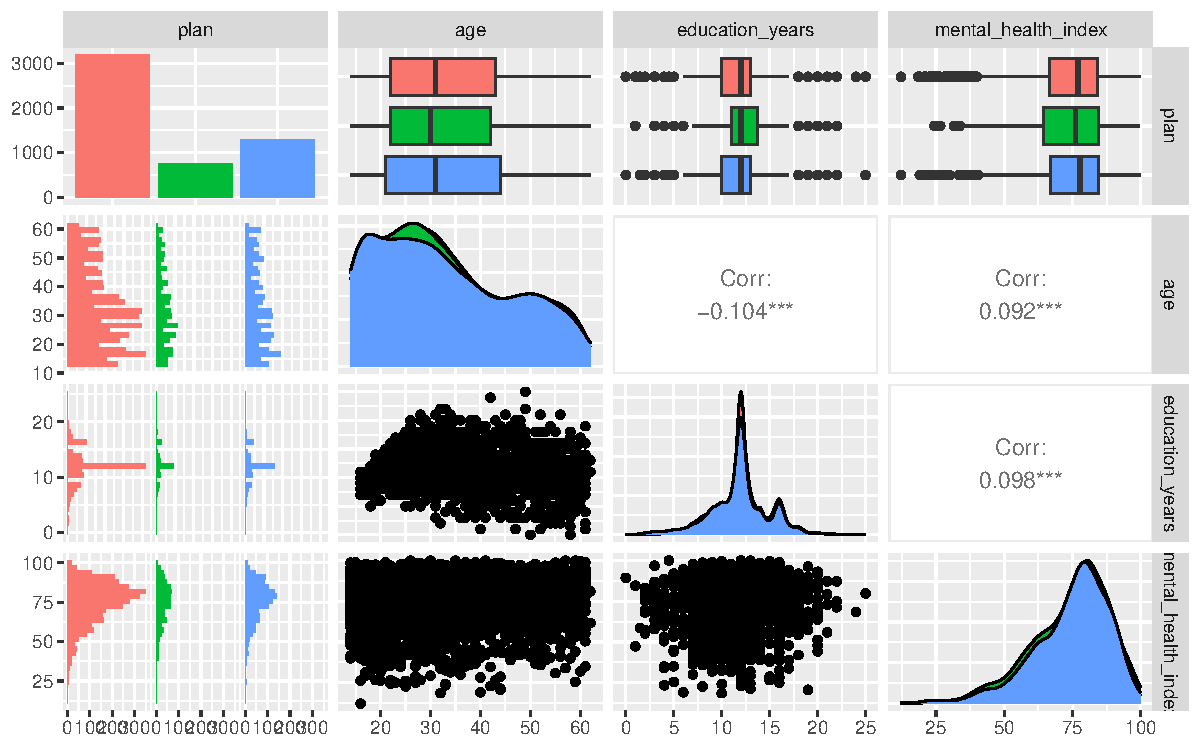
\includegraphics{RCT-RAND-HIE-part-2_files/figure-pdf/unnamed-chunk-14-1.pdf}

}

\end{figure}

\hypertarget{checks-and-balances}{%
\subsection{Checks and balances}\label{checks-and-balances}}

\hypertarget{means-differences-between-groups}{%
\subsubsection{Means differences between
groups}\label{means-differences-between-groups}}

We can perform means comparison tests one by one for each variable and
difference. For example:

\begin{Shaded}
\begin{Highlighting}[]
\FunctionTok{t.test}\NormalTok{(income\_family }\SpecialCharTok{\textasciitilde{}}\NormalTok{ plan, }\AttributeTok{data =}\NormalTok{ pre\_dta }\SpecialCharTok{\%\textgreater{}\%} \FunctionTok{filter}\NormalTok{(plan\_type\_2 }\SpecialCharTok{\%in\%} \FunctionTok{c}\NormalTok{(}\DecValTok{1}\NormalTok{,}\DecValTok{2}\NormalTok{)))}
\end{Highlighting}
\end{Shaded}

\begin{verbatim}

    Welch Two Sample t-test

data:  income_family by plan
t = 0.55359, df = 2285.9, p-value = 0.5799
alternative hypothesis: true difference in means between group Any insurance and group Free is not equal to 0
95 percent confidence interval:
 -820.0562 1465.1735
sample estimates:
mean in group Any insurance          mean in group Free 
                   30949.58                    30627.02 
\end{verbatim}

Make a similar comparison for a different plan type:

Make a similar comparison for a different outcome variable:

\hypertarget{checks-and-balances-tables}{%
\subsubsection{Checks and balances
tables}\label{checks-and-balances-tables}}

\texttt{datasummary\_balance()} is a more sophisticated function. It
builds summary statistics for multiple groups and for two groups only it
permits comparing means. For help, see \texttt{?datasummary\_balance}.

Compare leans for all variables across all insurances.

\begin{Shaded}
\begin{Highlighting}[]
\FunctionTok{datasummary\_balance}\NormalTok{(. }\SpecialCharTok{\textasciitilde{}}\NormalTok{ plan, }\AttributeTok{data =}\NormalTok{ pre\_dta)}
\end{Highlighting}
\end{Shaded}

\begin{verbatim}
Warning: These variables were omitted because they include more than 50 levels:
id.
\end{verbatim}

\begin{verbatim}
Warning: The difference in means can only be calculate with two groups in the
right-hand side variable. Set `dinm=FALSE` to suppress this warning.
\end{verbatim}

\begin{table}
\centering
\begin{tabular}[t]{lrrrrrr}
\toprule
\multicolumn{1}{c}{ } & \multicolumn{2}{c}{Any insurance (N=3198)} & \multicolumn{2}{c}{Catastrophic (N=759)} & \multicolumn{2}{c}{Free (N=1295)} \\
\cmidrule(l{3pt}r{3pt}){2-3} \cmidrule(l{3pt}r{3pt}){4-5} \cmidrule(l{3pt}r{3pt}){6-7}
  & Mean & Std. Dev. & Mean & Std. Dev. & Mean & Std. Dev.\\
\midrule
plantype & 1.9 & 0.8 & 4.0 & 0.0 & 1.0 & 0.0\\
female & 0.5 & 0.5 & 0.6 & 0.5 & 0.5 & 0.5\\
non\_white & 0.1 & 0.4 & 0.2 & 0.4 & 0.1 & 0.4\\
age & 33.0 & 13.3 & 32.4 & 12.9 & 32.8 & 13.5\\
education\_years & 11.9 & 3.0 & 12.1 & 2.9 & 11.8 & 3.1\\
income\_family & 30949.6 & 17286.8 & 31603.2 & 18148.3 & 30627.0 & 17201.1\\
hospitalization & 0.1 & 0.3 & 0.1 & 0.3 & 0.1 & 0.3\\
general\_health\_index & 69.9 & 15.0 & 70.9 & 14.9 & 69.6 & 15.0\\
cholesterol & 204.1 & 43.5 & 207.3 & 39.9 & 202.1 & 44.2\\
blood\_pressure & 123.7 & 16.6 & 122.3 & 16.5 & 123.5 & 16.3\\
mental\_health\_index & 74.6 & 13.8 & 73.8 & 14.3 & 74.7 & 13.9\\
plan\_type\_2 & 1.0 & 0.0 & 0.0 & 0.0 & 2.0 & 0.0\\
\bottomrule
\end{tabular}
\end{table}

Filter two insurance plans to compare means between those.

Filter other two insurance plans and compare means between them.

\hypertarget{mean-comparison-with-regression}{%
\subsubsection{Mean comparison with
regression}\label{mean-comparison-with-regression}}

Regression analysis could be used to compare means. For example:

\begin{Shaded}
\begin{Highlighting}[]
\NormalTok{mod1 }\OtherTok{\textless{}{-}} \FunctionTok{lm}\NormalTok{(income\_family }\SpecialCharTok{\textasciitilde{}}\NormalTok{ plan, }\AttributeTok{data =}\NormalTok{ pre\_dta)}
\FunctionTok{summary}\NormalTok{(mod1)}
\end{Highlighting}
\end{Shaded}

\begin{verbatim}

Call:
lm(formula = income_family ~ plan, data = pre_dta)

Residuals:
   Min     1Q Median     3Q    Max 
-31603 -13695  -1248  11376  57529 

Coefficients:
                 Estimate Std. Error t value Pr(>|t|)    
(Intercept)       30949.6      316.2  97.888   <2e-16 ***
planCatastrophic    653.6      722.8   0.904    0.366    
planFree           -322.6      588.3  -0.548    0.584    
---
Signif. codes:  0 '***' 0.001 '**' 0.01 '*' 0.05 '.' 0.1 ' ' 1

Residual standard error: 17390 on 4968 degrees of freedom
  (281 observations deleted due to missingness)
Multiple R-squared:  0.0002879, Adjusted R-squared:  -0.0001146 
F-statistic: 0.7153 on 2 and 4968 DF,  p-value: 0.4891
\end{verbatim}

\hypertarget{causal-effects}{%
\subsection{Causal effects}\label{causal-effects}}

To study causal effects, we will use a new data set, which loaded before
called: \texttt{post\_dta}.

Glimpse at it:

\begin{Shaded}
\begin{Highlighting}[]
\FunctionTok{glimpse}\NormalTok{(post\_dta)}
\end{Highlighting}
\end{Shaded}

\begin{verbatim}
Rows: 23,927
Columns: 9
$ person         <chr> "MA250247", "MA250247", "MA250247", "MA250247", "MA2502~
$ plan           <chr> "Free", "Free", "Free", "Free", "Free", "Free", "Free",~
$ year           <dbl> 1975, 1976, 1977, 1978, 1979, 1975, 1976, 1977, 1978, 1~
$ total_exp      <dbl> 36.3055, 275.2085, 0.0000, 0.0000, 0.0000, 0.0000, 0.00~
$ outpatient_exp <dbl> 36.3055, 275.2085, 0.0000, 0.0000, 0.0000, 0.0000, 0.00~
$ inpatient_exp  <dbl> 0, 0, 0, 0, 0, 0, 0, 0, 0, 0, 0, 0, 0, 0, 0, 0, 0, 0, 0~
$ admissions     <dbl> 0, 0, 0, 0, 0, 0, 0, 0, 0, 0, 0, 0, 0, 0, 0, 0, 0, 0, 0~
$ face_to_face   <dbl> 0, 4, 0, 0, 0, 0, 0, 1, 0, 0, 0, 2, 0, 0, 0, 7, 4, 0, 0~
$ plan_type_2    <dbl> 2, 2, 2, 2, 2, 2, 2, 2, 2, 2, 2, 2, 2, 2, 2, 2, 2, 2, 2~
\end{verbatim}

\hypertarget{t-test}{%
\subsubsection{t-test}\label{t-test}}

Use the t-test to show the effect of insurance on total expenditure on
healthcare.

\begin{Shaded}
\begin{Highlighting}[]
\FunctionTok{t.test}\NormalTok{(total\_exp }\SpecialCharTok{\textasciitilde{}}\NormalTok{ plan, }\AttributeTok{data =}\NormalTok{ post\_dta }\SpecialCharTok{\%\textgreater{}\%} \FunctionTok{filter}\NormalTok{(plan\_type\_2 }\SpecialCharTok{\%in\%} \FunctionTok{c}\NormalTok{(}\DecValTok{0}\NormalTok{,}\DecValTok{2}\NormalTok{)))}
\end{Highlighting}
\end{Shaded}

\begin{verbatim}

    Welch Two Sample t-test

data:  total_exp by plan
t = 5.2034, df = 8692, p-value = 2.001e-07
alternative hypothesis: true difference in means between group Catastrophic and group Free is not equal to 0
95 percent confidence interval:
 177.8311 392.8013
sample estimates:
mean in group Catastrophic         mean in group Free 
                  921.0358                   635.7196 
\end{verbatim}

\hypertarget{use-datasummary_balance-for-the-same-comparison}{%
\subsubsection{\texorpdfstring{Use \texttt{datasummary\_balance()} for
the same
comparison}{Use datasummary\_balance() for the same comparison}}\label{use-datasummary_balance-for-the-same-comparison}}

\begin{Shaded}
\begin{Highlighting}[]
\FunctionTok{datasummary\_balance}\NormalTok{(. }\SpecialCharTok{\textasciitilde{}}\NormalTok{ plan, }\AttributeTok{data =}\NormalTok{ post\_dta }\SpecialCharTok{\%\textgreater{}\%} \FunctionTok{filter}\NormalTok{(plan\_type\_2 }\SpecialCharTok{\%in\%} \FunctionTok{c}\NormalTok{(}\DecValTok{0}\NormalTok{,}\DecValTok{2}\NormalTok{)))}
\end{Highlighting}
\end{Shaded}

\begin{verbatim}
Warning: These variables were omitted because they include more than 50 levels:
person.
\end{verbatim}

\begin{table}
\centering
\begin{tabular}[t]{lrrrrrr}
\toprule
\multicolumn{1}{c}{ } & \multicolumn{2}{c}{Catastrophic (N=6840)} & \multicolumn{2}{c}{Free (N=3724)} & \multicolumn{2}{c}{ } \\
\cmidrule(l{3pt}r{3pt}){2-3} \cmidrule(l{3pt}r{3pt}){4-5}
  & Mean & Std. Dev. & Mean & Std. Dev. & Diff. in Means & Std. Error\\
\midrule
year & 1977.7 & 1.6 & 1977.5 & 1.7 & -0.2 & 0.0\\
total\_exp & 921.0 & 2959.6 & 635.7 & 2535.3 & -285.3 & 54.8\\
outpatient\_exp & 416.9 & 620.7 & 247.8 & 487.6 & -169.1 & 11.0\\
inpatient\_exp & 504.1 & 2705.5 & 387.9 & 2308.1 & -116.2 & 50.0\\
admissions & 0.1 & 0.4 & 0.1 & 0.4 & 0.0 & 0.0\\
face\_to\_face & 4.4 & 7.4 & 2.8 & 5.5 & -1.7 & 0.1\\
plan\_type\_2 & 0.0 & 0.0 & 2.0 & 0.0 & 2.0 & 0.0\\
\bottomrule
\end{tabular}
\end{table}



\end{document}
